\documentclass{article}
\usepackage[UTF8]{ctex}
\usepackage{CJKutf8}
\usepackage{color}
\usepackage{natbib}
\usepackage{graphicx}
\usepackage{subfigure}
\usepackage{geometry}
\usepackage{amsmath}
\usepackage{mathrsfs}
% java code settings
\usepackage{listings}
\usepackage{xcolor}
\definecolor{dkgreen}{rgb}{0,0.6,0}
\definecolor{gray}{rgb}{0.5,0.5,0.5}
\definecolor{mauve}{rgb}{0.58,0,0.82}
\lstset{frame=tb,
     language=Java,
     aboveskip=3mm,
     belowskip=3mm,
     showstringspaces=false,
     columns=flexible,
     basicstyle = \ttfamily\small,
     numbers=none,
     numberstyle=\tiny\color{gray},
     keywordstyle=\color{blue},
     commentstyle=\color{dkgreen},
     stringstyle=\color{mauve},
     breaklines=true,
     breakatwhitespace=true,
     tabsize=3
}
\geometry{a4paper, scale=0.8}

\title{\textbf{EE447 Lab3 \\ QR Code Report}}
\author{付昊源 517021910753}
\date{May 5, 2020}

\begin{document}

\maketitle

%%%%%%%%%%%%%%%%%%%%%%%%%%%%%%
\section{Lab Overview}
QR code, which stands for Quick Response code, is the most popular encoding method on mobile devices in recent years. It can store more information than traditional barcode as well as more data types. The QR code system becomes popular outside the automotive industry due to its fast readability and greater storage capacity compared to standard UPC barcodes. A QR code consists of black square dots arranged in a square grid on a white background and it can be scanned by camera, scanner, etc. There are also other algorithms such as Reed-Solomon error correction to let the image appropriately interpreted. Other QR codes with more colors than black and white, and dynamic QR codes store much more information than standard black and white QR codes.

In this lab, we will develop an application with the capability of QR code encoding and decoding on android device. Actually, the codes have been well-written, but its android SDK version and gradle version fuse me a lot. I spent most time solving the errors about environment. So in this report, I will first summarize the problems I met and corresponding solutions. Then, I will introduce the work flow of this app with my own understanding.

\section{Lab Procedure}
In this section, I will first summarize the problems I met. All problems are about android SDK version, SDK build-tools version and gradle scripts. I will also present the effective solutions for each problem. Finally, I will introduce how the codes work with my own understanding.

\subsection{Problems and Solutions}
\subsubsection{Could not run build action using Gradle distribution xxx}
First I want to say, not everyone may meet this problem. When this android project is loaded, Android Studio will automatically synchronize the project and modules. It will check the distributionUrl in \textit{gradle-wrapper.properties} and download the target version of gradle if there isn't a available version in your computer.

\begin{figure}[htbp]
     \centering
     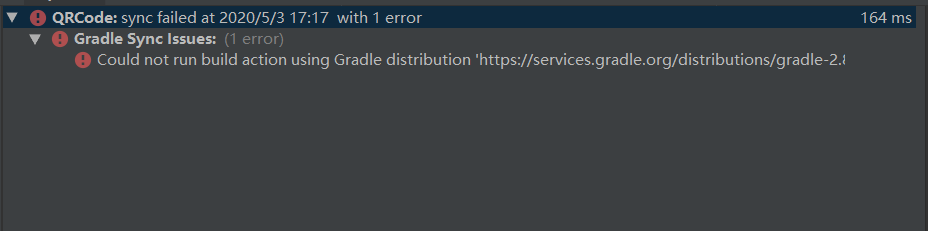
\includegraphics[width=\linewidth]{error1.jpg}
     \caption{Error: Could not run build action using Gradle distribution xxx.}
\end{figure}

However, in the first time I loaded this project, my network broke down and there may lose some packages. After fixing the network and load it again, due to the incompletion of gradle, this problem 'Could not run build action using gradle distribution xxx' occurs.

There are many solutions about this problem on the internet, but many of them are wrong. Since we know the reason of this problem is broken gradle, we must download it again. However, only deleting the gradle folders in root
$$C:\backslash User\backslash \$UserName\$\backslash .gradle\backslash wrapper\backslash dists$$
cannot work. This is because Android Studio also preserves some cache files and we must delete them together. So the effective method is to delete all files and folders in
$$C:\backslash User\backslash \$UserName\$\backslash .gradle$$
Though this may affect other android projects, but Android Studio will help you download them when you load this project again. After these, start from scratch.

\subsubsection{Failed to find Build Tools revision 23.0.1}
This problem occurs when you didn't install the SDK build tools with the target version 23.0.1. Here let's talk about the compile SDK version and SDK build tools version.

First please open file build.gradle(Module:app) in Gradle Scripts in Android Studio. You may see two lines like this
\begin{lstlisting}[language=Java]
     compileSdkVersion 21
     buildToolsVersion "23.0.1"
\end{lstlisting}
The upper line is about Android SDK tool and the second line is about SDK build tool. We must check our own SDK manager and make it match the two lines above.

For Android SDK tool, a higher version can satisfy the requirements of a lower version. Most of us installed Android SDK tools 26, which is greater than 21, so this is OK. However, SDK build tool version must be exactly the same. You can open your SDK manager to check whether you have downloaded and installed build tool 23.0.1. If you have not installed it, this problem occurs. To fix it, just download and install manually, then try again.

\subsubsection{Failed to resolve: com.android.support:appcompact-v7:21.0.3}
\begin{figure}[htbp]
     \centering
     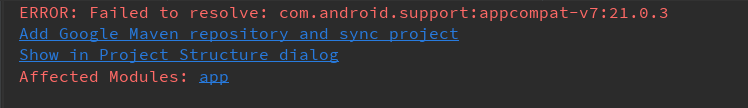
\includegraphics[width=\linewidth]{error2.PNG}
     \caption{Error: Failed to resolve: com.android.support:appcompact-v7:21.0.3.}
\end{figure}
I think nearly everyone may meet this problem because we cannot resolve this package locally. So we should add some maven url into file \textit{build.gradle(Project: QRCode)}. However, due to the version of gradle in this project is 2.8, many online solutions cannot work. The easiest and safest way to fix this error is to click the option 'Add Google Maven repository and sync project' in Figure 2. Then it will show things like Figure 3
\begin{figure}[htbp]
     \centering
     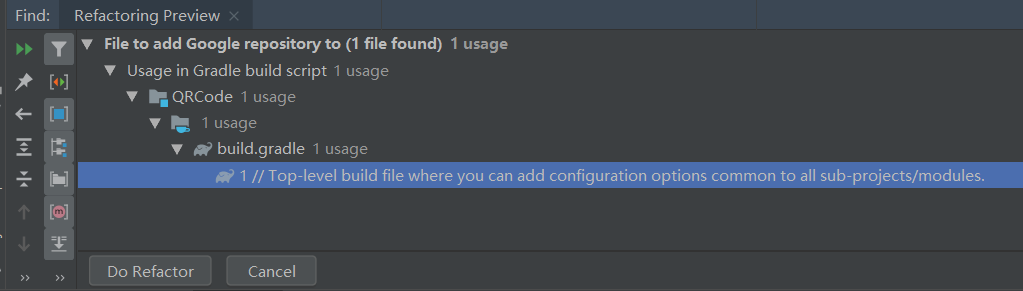
\includegraphics[width=\linewidth]{error3.PNG}
     \caption{Further options about fixting Error in Figure 2.}
\end{figure}

Finally, click 'Do Refactor' at the left-bottom corner in Figure 3 to fix this problem. If nothing unexpected happens, this project will be synchronized and build successfully. Then you can extract the apk into mobile phone and test this application.

\subsection{Understanding Codes}
There are three main activities, MainActivity, TestDecoder and TestEncoder.
\subsubsection{MainActivity}
In MainActivity, we override two functions: onCreate() and onActivityResult(). The first function is not strange since we have used it many times, but the second function is seen here for the first time. Function onActivityResult() is to get the response from some other triggers or message passing. In this application, it responds from TestDecoder when meeting a valid QR code. TestDecoder send the decoding result back and MainActivity make a AlterDialog to show the result.

Function onCreate() here is quite simple, it just creates an OnClickListener to listen the operation of button encoder and decoder. If either button is pushed, it will execute the corresponding work. But notice that if we push the decoder button, the activity need result so it uses startActivityForResult() instead of startActivity().

\subsubsection{TestEncoder}
In TestEncoder, most work have been done in library zxing. What we need to do is getting text from the EditText module, and send the text into parameter of API MultiFormatWriter(). It will return a bitMatrix representing each pixel's black or white. We just convert it into RGB color and draw those pixels on a bitmap. Finally, paste the bitmap on an ImageView and put this view onto an AlterDialog to show the encoding result. The outcome is shown in Figure 4(a).

\begin{figure}[htbp]
     \centering
     \subfigure[TestEncoder working screenshot on real mobile phone.] {
         \begin{minipage}[t]{0.4\linewidth}
             \centering
             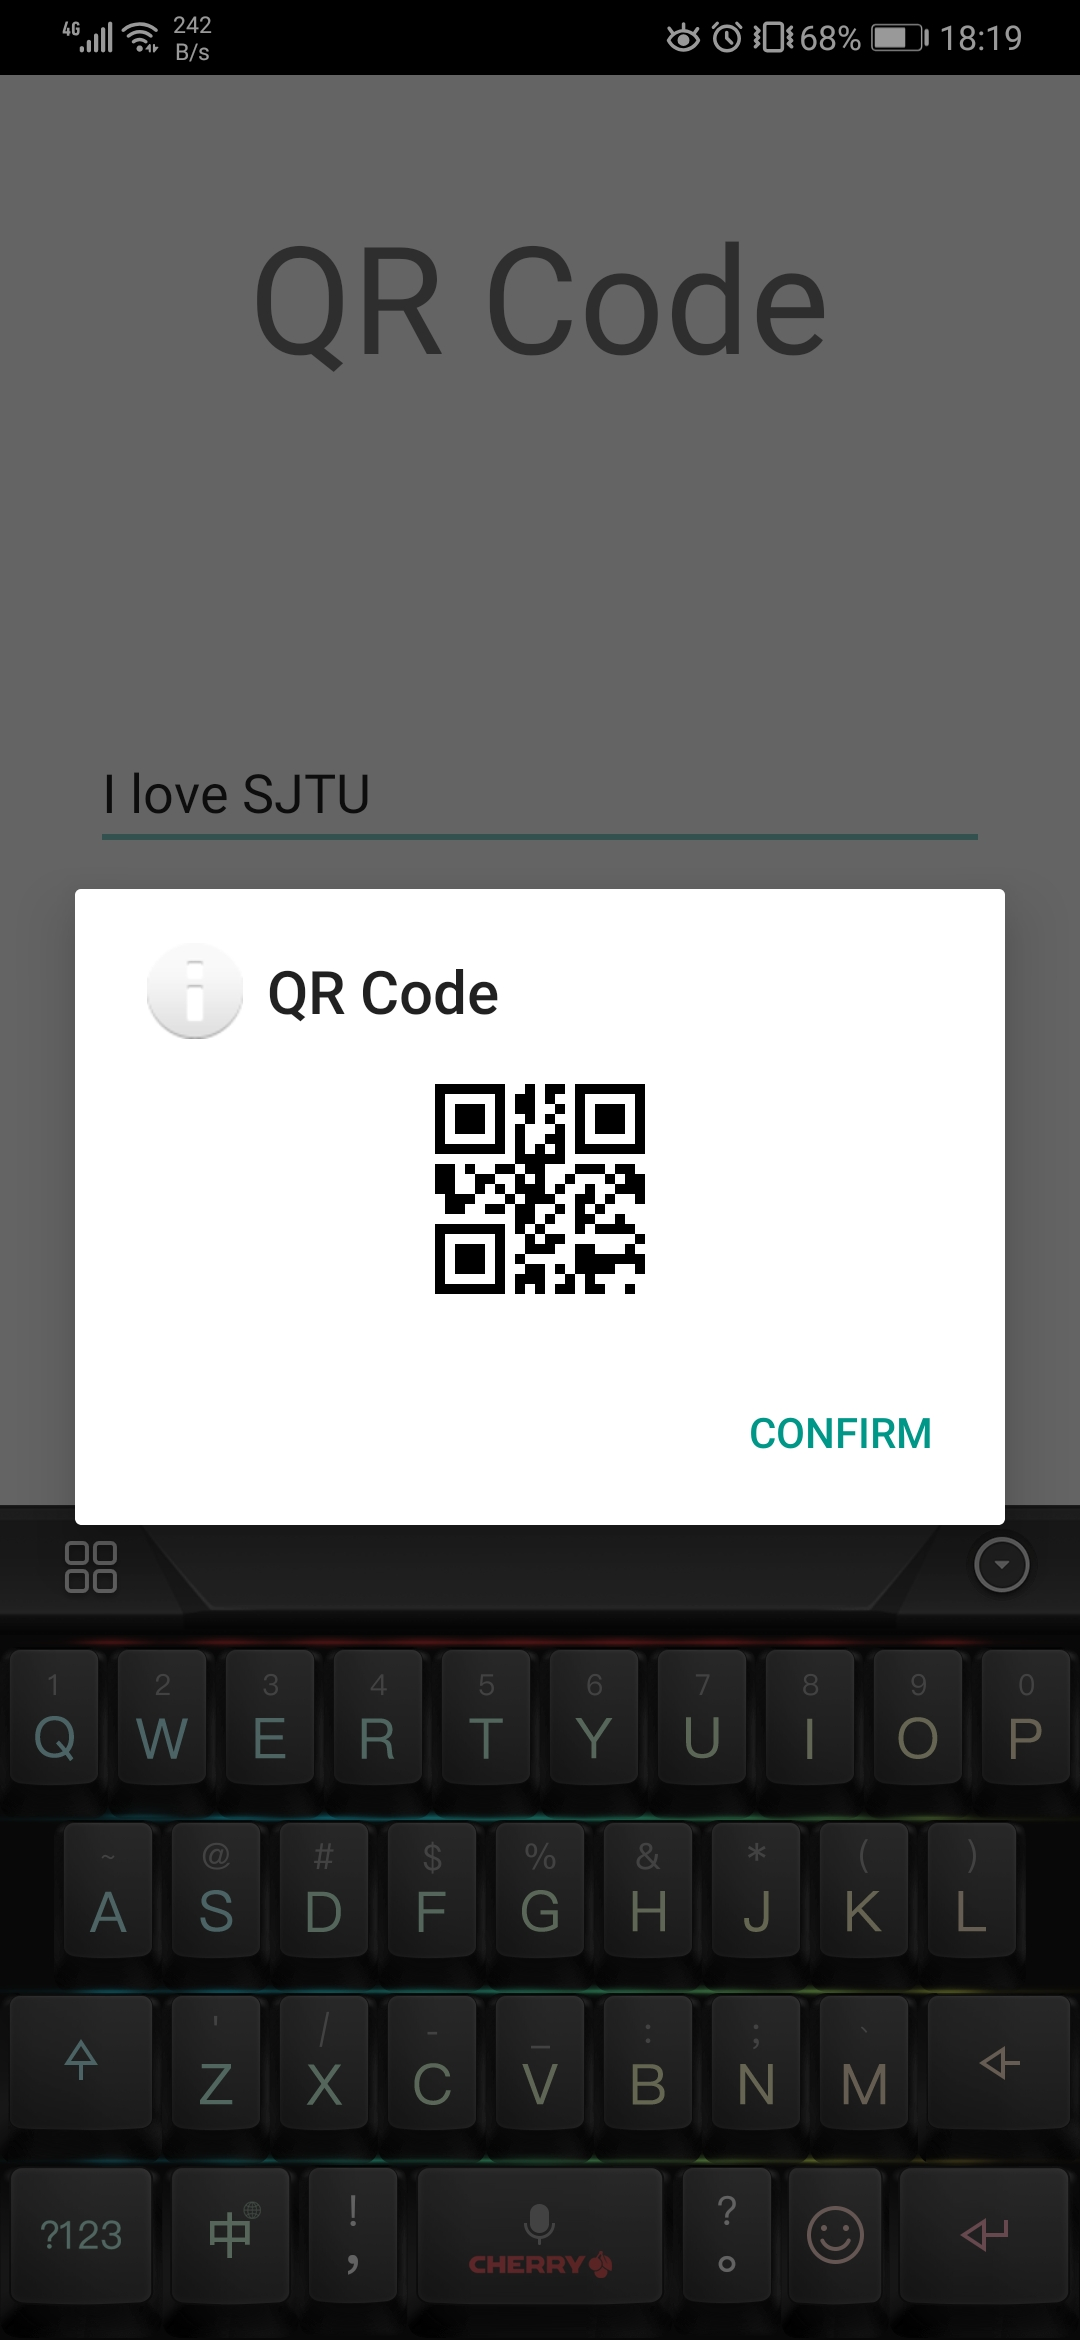
\includegraphics[width=\linewidth]{screenshot1.jpg}
         \end{minipage}
     }
     \subfigure[TestDncoder working screenshot on real mobile phone. The QR code I scanned is for wechat login.]{
         \begin{minipage}[t]{0.4\linewidth}
             \centering
             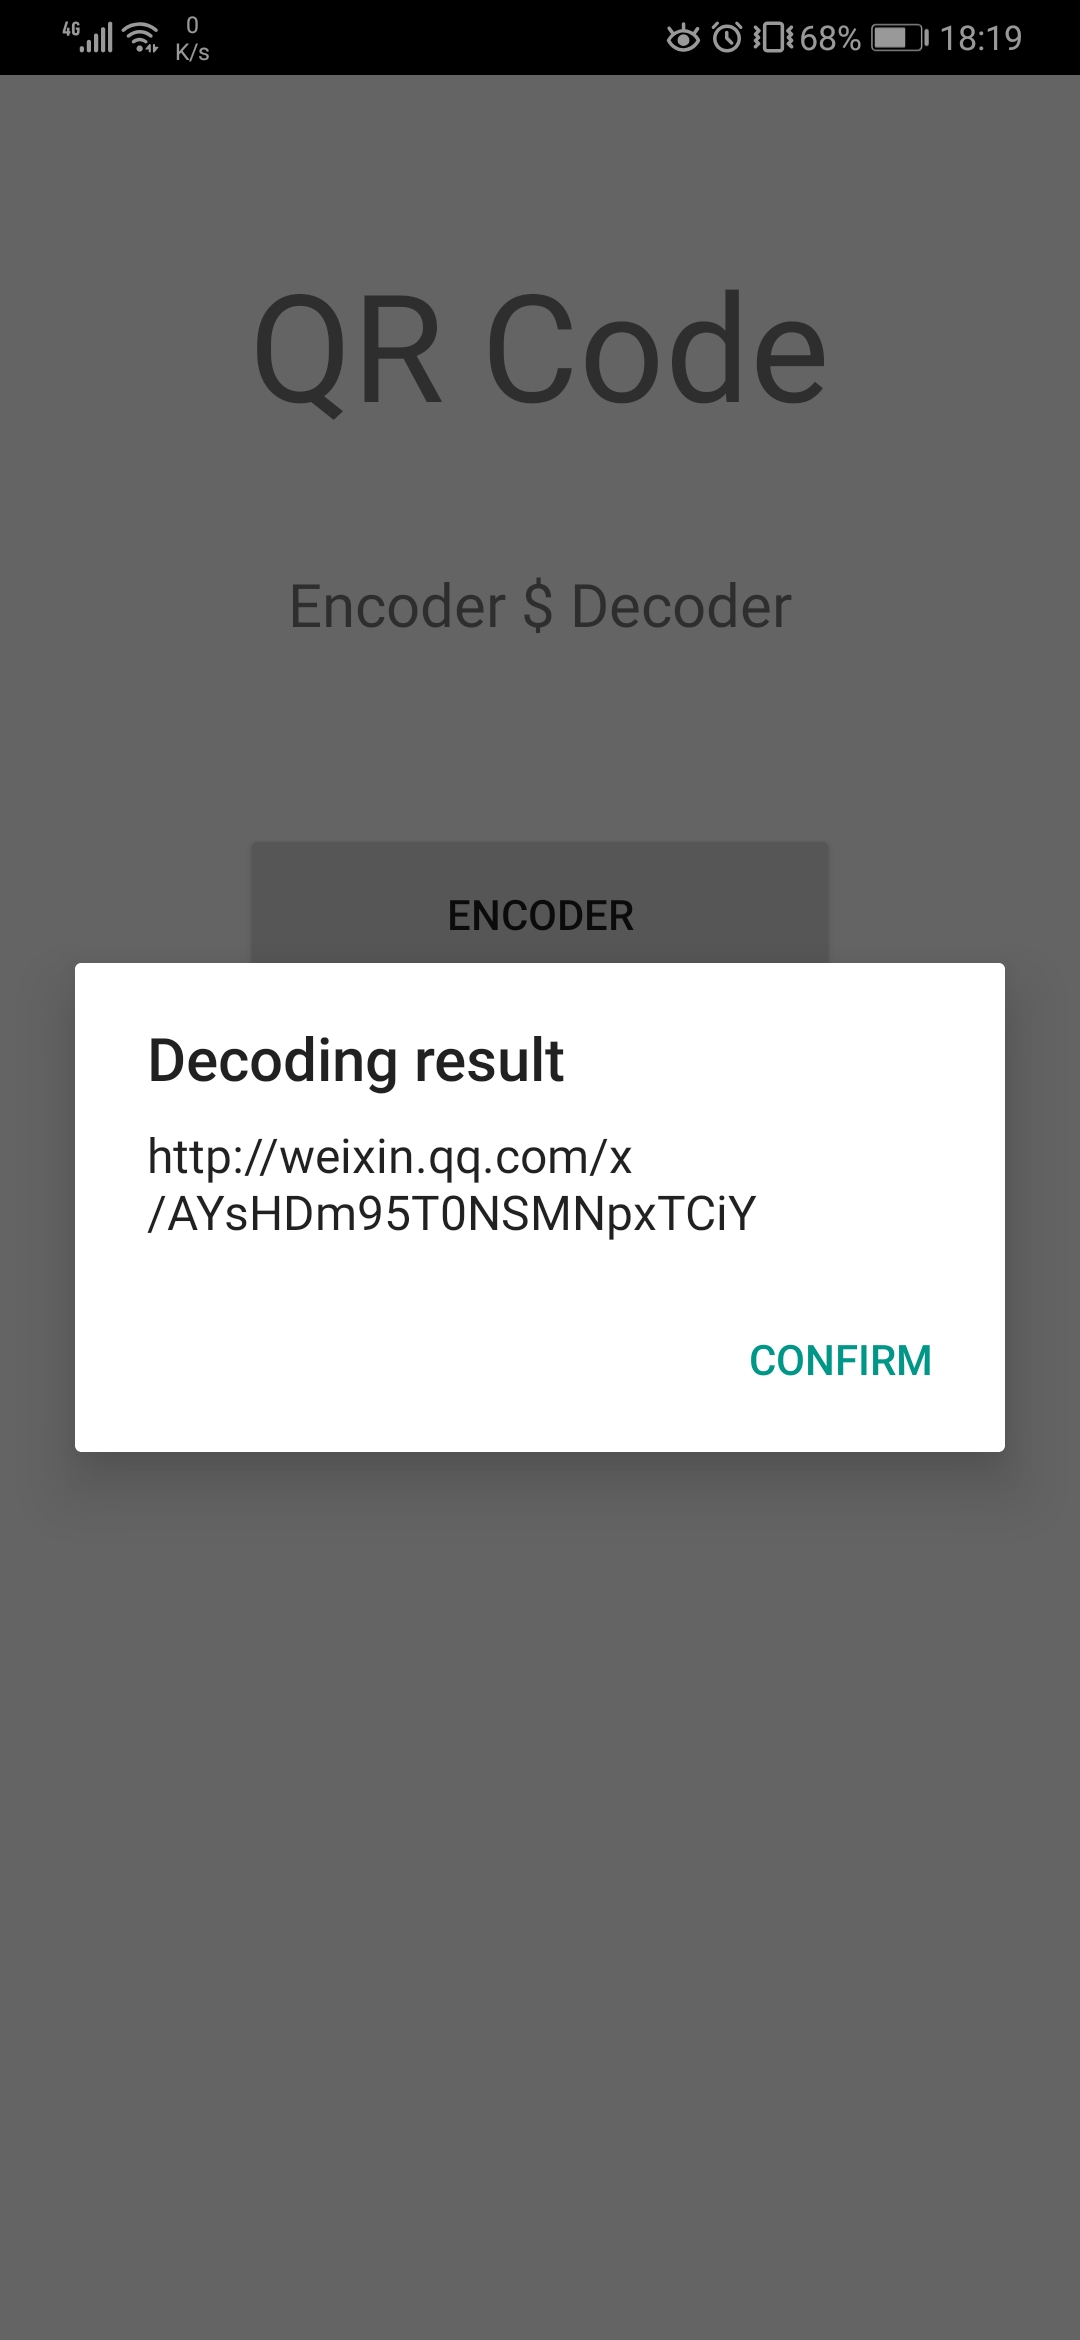
\includegraphics[width=\linewidth]{screenshot2.jpg}
         \end{minipage}
     }
     \caption{Screen shots of Measurement of WiFi Signal Strength on real mobilephone}
\end{figure}

\subsubsection{TestDecoder}
In TestDecoder, this class implements SurfaceHolder.Callback. So it must have three functions: surfaceCreated(), surfaceChanged() and surfaceDestroyed(). The first one is called when SurfaceView is first created. The second one is called when SurfaceView's size and format is changed. The last one is called when SurfaceView is destroyed. The screen shot of decoder is shown at Figure 4(b). And in this subsubsection, I will introduce the process of this activity.

Let's start from onCreate() function. When this activity is first created, we want it to be a surfaceView with the whole screen being camera result. Thus, we need to initialize the surfaceView and bonding it to a surfaceHolder. During this procedure, surfaceCreated() function is used automatically. Actually, the three functions mentioned in the last paragraph is regarded as callback functions, and they are inserted into surfaceHolder.

In surfaceCreated(), we first open the camera and accept camera images. For each frame, translate the image to a bitmap pass it to a QRCodeReader. The reader continuously reads and parses the image data and try to extract real QR code from the image. If a QR code is found, the reader will decode the result, insert it into bundle and send back to MainActivity. If not found, the reader will skip the current frame and check the next frame, until a valid QR code is really found and decoded.

In surfaceChanged() function, we need to initialize camera in the format of changed size by calling initCamera(). This function is long, but most codes are for logging information. It mainly get the parameters of changed size camera and set some hyper parameters for this camera such as JPEG format, picture size, and focus mode. Besides, it also set the display orientation. Finally, start preview and we will see what camera scans.

Finally, when the surface is destroyed, surfaceDestroyed() is called. Note that we must set preview callback function to \textit{null} fist. Otherwise, the program will crash. Then, stop previewing and release the camera object. All these will be automatically called when finish() is called. So it's just like a destructor in a class.

\section{Conlusion and Future Work}
In this lab, we design a QR code encoder and decoder into one application. During the encoder stage, we just rely on a third-party library \textit{zxing} to encode input string into a QR code. In decoder stage, we need the authority of camera. After getting the photo from camera, \textit{zxing} will parse the photo, check the possible QR code and decode it. Finally, it will return a result with decoded string back to main activity.

The process is clear and easy to understand, but since the codes are not written by myself, I hope to modify some of the codes and implement new functions. There are some functions like, visulizing the localizathion of the QR code when there are muliple QR codes in a photo; decoding multiple QR codes and return all the result strings. This may be hard since we may need to modify \textit{zxing} source code, but for future work, I want to try this.
%%%%%%%%%%%%%%%%%%%%%%%%%%%%%%

\end{document}
